\section{Teoria dos Grafos e Redes Complexas} \label{sec:graphtheory}

Grafos são constructos matemáticos compostos por pontos, denominados vértices ou nós, que podem estar conectados por linhas, denominadas arestas ou arcos, dependendo da presença ou ausência de direção nas mesmas \cite{Bondy1976}. Tais objetos podem ser empregados na representação de uma grande variedade de situações e problemas reais, como cadeias alimentares ou redes tróficas, o conjunto de vasos sanguíneos de um corpo, redes metabólicas, complexos de proteínas, redes neurais biológicas, redes de colaboração entre pesquisadores, relações de negócio entre corporações, redes ferroviárias e a própria Internet, além de outros exemplos \cite{Newman2003}.

Naturalmente, grafos também podem ser utilizados para representar redes sociais, exploradas na Seção \ref{sec:socialnetworks}, de forma muito conveniente: os vértices do grafo representam atores, enquanto as arestas ou arcos simbolizam os laços entre os mesmos \cite{Newman2003}. Desta maneira, é possível apropriar-se de grande parte da literatura da Teoria dos Grafos no desenvolvimento de estudos sobre redes sociais, favorecendo uma compreensão mais concreta de seus conceitos matemáticos abstratos.

A definição de grafos é essencialmente genérica, isto é, não há nenhuma suposição quanto a existência ou não de padrões formados por suas arestas ou quanto à qualquer característica de seus vértices. Adicionalmente, não há nenhuma delimitação quanto ao número de vértices ou arestas presentes no grafo; por consequência, um grafo pode possuir 10 vértices e nenhuma aresta, ou um vértice e 10 arcos ligando-o a si próprio (um tipo de arco conhecido na literatura como laço reflexivo\footnote{tradução livre de \textit{self-loop}}), ou até mesmo uma quantidade infinita de vértices e arestas, formando um grafo infinito \cite{Bondy1976}.

Entretanto, dada a ubiquidade da modelagem de sistemas e situações reais como grafos, definiu-se o termo \emph{Rede Complexa} para denominar grafos cujas topologias apresentam características similares a redes observáveis no mundo real, onde ordem e desordem coexistem \cite{Fortunato2010}. Sendo assim, um grafo aleatório formado a partir do modelo de \citeonline{Erdos1959} não pode ser considerado uma rede complexa, por apresentar alto índice de homogeneidade na distribuição de suas arestas, enquanto a rede social do clube de karatê, apresentada na Figura \ref{fig:karate}, pode ser considerada um exemplo típico de rede complexa.

O presente trabalho aborda exclusivamente redes sociais, e portanto fará uso principalmente da literatura científica acerca de redes complexas, visto que a grande maioria das redes sociais são instâncias de redes complexas. Consequentemente, verifica-se a necessidade de esclarecer a seguinte hierarquia de nomenclaturas, em ordem de especificidade crescente:

\begin{alineas}
    \item Grafo: empregado ao tratar de assuntos que se aplicam a qualquer arranjo de vértices e arestas, especialmente em contextos matemáticos;
    \item Rede complexa: termo utilizado na discussão de grafos com topologia não-trivial, com características observáveis comumente no mundo real;
    \item Rede social: especialização de rede complexa, onde vértices representam atores (indivíduos) e arestas representam laços (relacionamento interpessoal de qualquer natureza).
\end{alineas}

A Figura \ref{fig:networknomenclature} apresenta uma demonstração gráfica da distinção entre estes três termos, onde: o grafo (a) consiste em um arranjo puramente arbitrário com propriedades matemáticas particulares \cite{Bondy1976}; a rede complexa (b) consiste em um conjunto de páginas da \textit{web} com arcos representando os \textit{hyperlinks} entre as páginas \cite{Fortunato2010}; e a rede social (c) consiste em uma rede de co-autoria de artigos científicos na área de detecção de comunidades em redes complexas \cite{Newman2004}.

\begin{figure}[ht]
    \centering
    \begin{subfigure}{0.36\textwidth}
        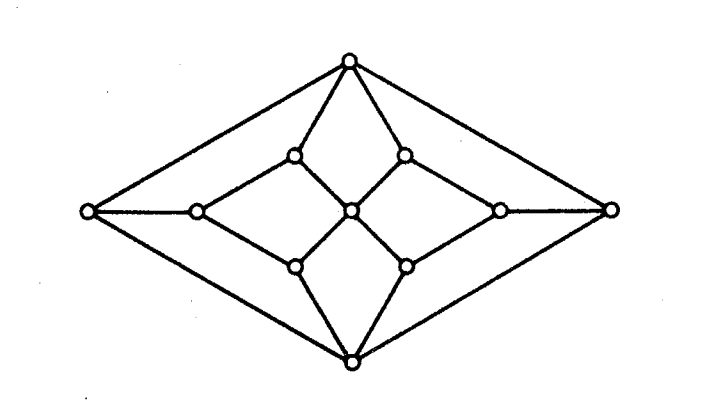
\includegraphics[width=\linewidth]{imagens/generic_graph.png}
        \caption{Grafo} \label{fig:1a}
    \end{subfigure}
    \vspace*{0.2cm}
    %\hspace*{\fill} % separation between the subfigures
    \begin{subfigure}{0.31\textwidth}
        \includegraphics[width=\linewidth]{imagens/complex_network2.png}
        \caption{Rede Complexa} \label{fig:1b}
    \end{subfigure}
    \\
    %\hspace*{\fill} % separation between the subfigures
    \begin{subfigure}{0.54\textwidth}
        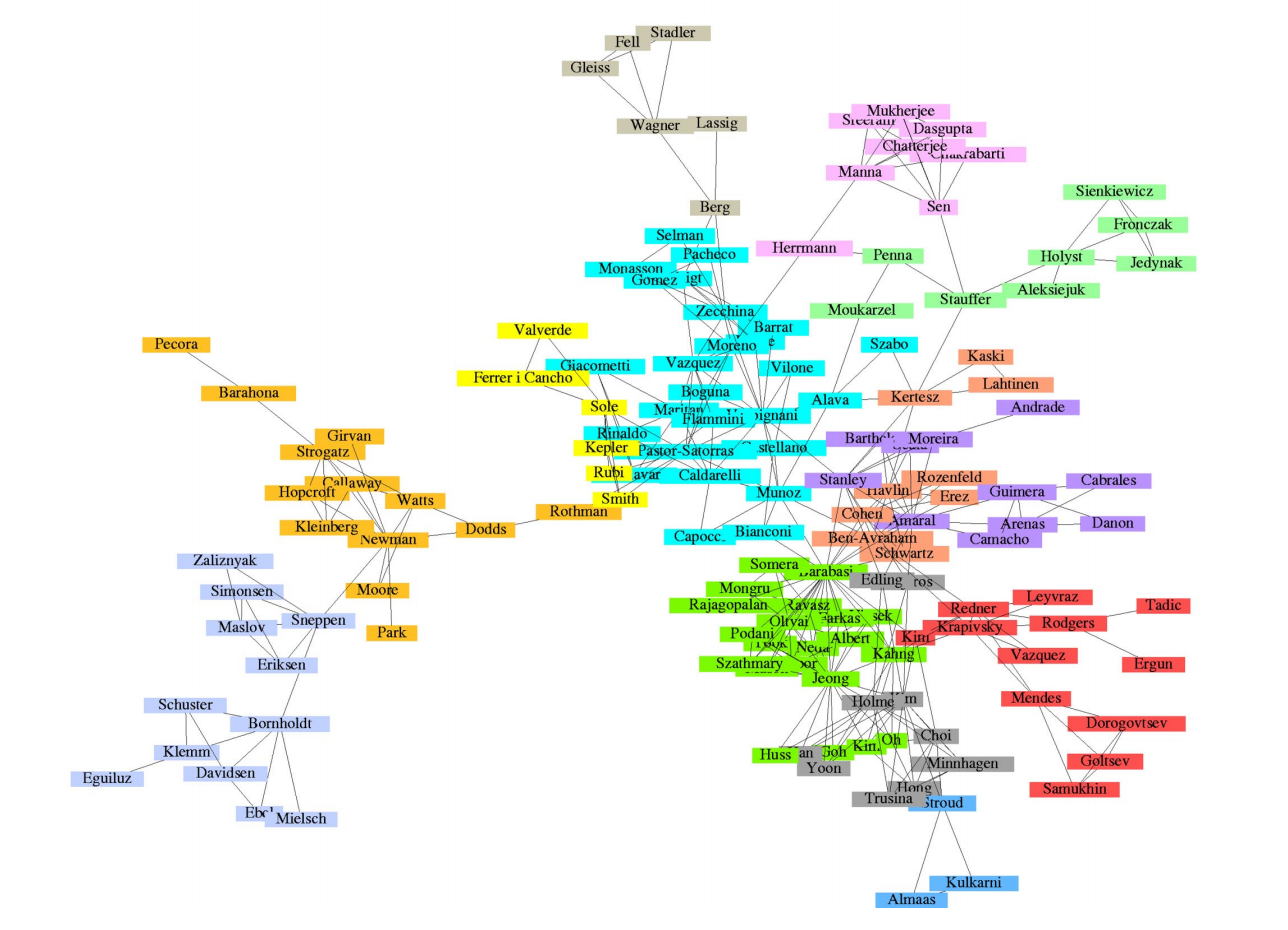
\includegraphics[width=\linewidth]{imagens/collaboration_network.png}
        \caption{Rede Social} \label{fig:1c}
    \end{subfigure}
    \vspace*{0.3cm}
    \caption{Distinção entre nomenclaturas}
    \label{fig:networknomenclature}
    \Fonte{Adaptado de \citeonline{Bondy1976}, \citeonline{Fortunato2010} e \citeonline{Newman2004}.}
\end{figure}

\subsection{Conceitos Fundamentais} \label{sec:graphfoundation}

Segundo \citeonline{Harary1969}, a terminologia e notação matemática empregadas na descrição de grafos varia frequentemente de trabalho para trabalho; portanto, é sugerido que cada autor esclareça com antecedência de que forma um grafo será descrito. Neste estudo, grafos serão tratados como pares $G = (V, E)$, onde $V$ consiste no conjunto de vértices, e o conjunto $E$ representa as arestas do grafo, composto por pares de nós $\{u, v\}$.

Caso as arestas do grafo possuam direção -- ou seja, se a aresta entre $u$ e $v$ for independente da aresta entre $v$ e $u$ --, terá-se um grafo dirigido, onde o termo ``arestas'' e seu conjunto $E$ é substituído por ``arcos'', os quais são representados por um conjunto $A$ de pares ordenados $(u, v)$. Em grafos dirigidos, um arco de $u$ até $v$ pode ser completamente diferente do arco na direção oposta, de $v$ até $u$; além disso, um deles pode existir sem o outro. O termo ``ligação'' será utilizado para referir-se a arcos e arestas de forma indistinta, assim como o termo ``laço'' (equivalente) foi utilizado na Seção \ref{sec:socialnetworks}.

Ao longo de toda a extensão deste trabalho, todos os grafos estudados serão simples; isto é, entre quaisquer vértices $u$ e $v$, pode existir somente uma ou nenhuma aresta $\{u, v\}$ ou, caso o grafo seja dirigido, pode existir nenhum arco, um arco $(u, v)$, um arco $(v, u)$, ou ambos os arcos. Além disso, não são permitidos \textit{loops} ou laços reflexivos, onde uma ligação possui origem igual ao seu destino. Grafos que permitem \textit{loops} e múltiplas ligações entre dois vértices são denominados multigrafos \cite{Newman2010}.

Além de simplesmente existirem ou não, ligações podem possuir um valor associado, denominado peso. Este valor pode representar uma grande variedade de conceitos, como distância entre cidades, a largura de banda entre dois pontos de rede, a impedância ou corrente entre duas extremidades em um circuito elétrico ou a frequência de contato ou amizade entre dois indivíduos (atores) \cite{Newman2010}. Caso as ligações possuam peso, o grafo é denominado ponderado.

A literatura da Teoria dos Grafos define diversos outros termos, com diferentes níveis de especificidade. Alguns destes, selecionados por apresentarem maior relevância neste estudo, são definidos da seguinte forma:

\begin{alineas}
    \item Grau: para um vértice $u$, seu grau é definido como a quantidade de vértices ligados a $u$ por uma aresta. Em grafos dirigidos, o grau se divide em grau de entrada (arcos com destino em $u$) e grau de saída (arcos com origem em $u$);
    \item Subgrafo: um grafo $G'$ derivado de $G$ cujo conjunto de vértices $V'$ consiste em um subconjunto de $V$. As ligações de $G'$ podem existir somente entre os vértices de $V'$;
    \item Grafo completo: um grafo onde, para todos os vértices $u$ e $v$, existe uma aresta $\{u, v\}$ ou, caso o grafo seja dirigido, ambos os arcos $(u, v)$ e $(v, u)$ estão presentes. Em outras palavras, todos os vértices estão ligados a todos os outros. Grafos completos são tipicamente denominados $K_n$, com $n = |V|$ (número de vértices);
    \item Clique: um subgrafo de $G$ que, tomado de forma isolada, consiste em um grafo completo; % talvez não precise
    \item Caminho: uma sequência de vértices com origem em $u$ e destino em $v$ tal que cada vértice da sequência está conectado ao próximo por uma ligação. A distância do caminho é igual ao somatório dos pesos das ligações\footnote{caso o grafo seja não-ponderado, considera-se que o peso da ligação é igual a 1.}. Caso não exista nenhum outro caminho entre $u$ e $v$ com distância menor, tem-se um caminho denominado \emph{caminho mínimo};
    \item Matriz de adjacências: representação matemática de um grafo, que consiste em uma matriz quadrada de ordem dada por $|V|$. Cada célula indica se existe ou não uma aresta ou arco entre os vértices representados pela combinação de linha (origem) e coluna (destino). Caso não haja ligação, a célula terá valor 0; caso contrário, o valor será o peso da ligação ou 1. Em grafos simples, a diagonal principal é sempre composta por zeros.
\end{alineas}

\subsection{Centralidade} \label{sec:centrality}

Segundo \cite{Newman2010}, há um volume expressivo de estudos referentes ao conceito de centralidade em redes complexas. Em linhas gerais, a medida de centralidade busca identificar quais são os vértices mais importantes em uma rede complexa; no entanto, a própria definição de ``importante'' é subjetiva e aberta a questionamentos, e consequentemente diversas métricas de centralidade foram desenvolvidas ao longo das décadas recentes.

Historicamente, a centralidade tem sido estudada principalmente no contexto de redes sociais \cite{Bavelas1948,Newman2010}; no entanto, aplicações em outras áreas também vem sendo publicadas, como em rotas de comércio no planejamento urbano \cite{Pitts1965}, redes de citação e colaboração científica \cite{Newman2001} e disseminação de epidemias \cite{Santiago2019}. % Revisar a citação e colaboração científica (é social em teoria)

O Quadro \ref{board:centralities} enumera algumas das principais métricas de centralidade, identificando seus conceitos ou ideias gerais de forma breve de acordo com autores da área \cite{Newman2010,Grando2015}.


\begin{quadro}[ht]
    \caption{Sumário de métricas de centralidade}
    \label{board:centralities}
    \fontsize{10}{12}\selectfont
    \def\arraystretch{1.25}
    \begin{tabularx}{\textwidth}{|c|c|Y|}
        \hline
        \textbf{Métrica} & \textbf{Tradução livre} & \textbf{Conceito}
        \\ \hline
        \textit{Degree Centrality} & Grau & Visibilidade, atividade de comunicação
        \\ \hline
        \textit{Betweenness Centrality} & Intermediação & Controle de comunicação, ação como ponte
        \\ \hline
        \textit{Closeness Centrality} & Proximidade & Independência, eficiência
        \\ \hline
        \textit{Eigenvector Centrality} & Autovalor & Importância proporcional à importância dos contatos
        \\ \hline
        \textit{Katz Centrality} & -- & Variante de Autovalor com um parâmetro constante. Mais apropriada para grafos dirigidos
        \\ \hline
    \end{tabularx}
\end{quadro}

Visando habilitar uma compreensão mais ampla sobre as cinco métricas de centralidade descritas, a Figura \ref{fig:centralities} apresenta visualmente cada uma delas aplicadas sobre uma rede complexa arbitrária. Cores azuis representam centralidade baixa, enquanto cores tendendo ao vermelho escuro indicam centralidade alta.

\begin{figure}[ht]
    \centering
    \vspace*{0.4cm}
    \begin{subfigure}{0.27\textwidth}
        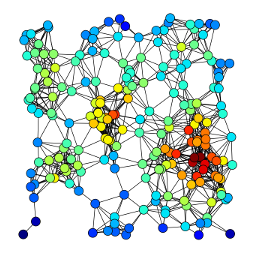
\includegraphics[width=\linewidth]{imagens/degree.png}
        \caption{Grau} \label{fig:degree}
    \end{subfigure}
    \begin{subfigure}{0.27\textwidth}
        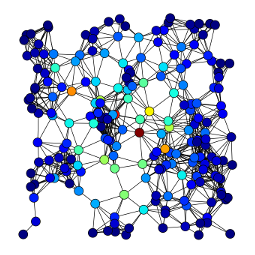
\includegraphics[width=\linewidth]{imagens/betweenness.png}
        \caption{Intermediação} \label{fig:betweenness}
    \end{subfigure}
    \begin{subfigure}{0.27\textwidth}
        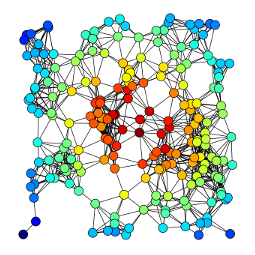
\includegraphics[width=\linewidth]{imagens/closeness.png}
        \caption{Proximidade} \label{fig:closeness}
    \end{subfigure}
    \\
    \vspace*{0.2cm}
    %\hspace*{\fill} % separation between the subfigures
    \begin{subfigure}{0.27\textwidth}
        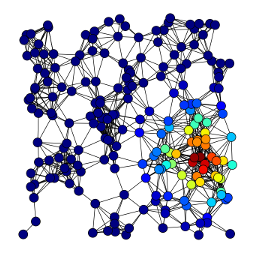
\includegraphics[width=\linewidth]{imagens/eigenvector.png}
        \caption{Autovalor} \label{fig:eigenvector}
    \end{subfigure}
    \begin{subfigure}{0.27\textwidth}
        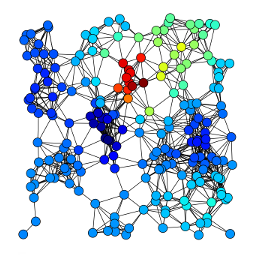
\includegraphics[width=\linewidth]{imagens/katz.png}
        \caption{Katz} \label{fig:katz}
    \end{subfigure}
    
    \vspace*{0.3cm}
    \RaggedRight
    \caption{Visualização de métricas de centralidade.}
    \label{fig:centralities}
    \Fonte{Wikimedia Commons}
\end{figure}

\subsubsection{Grau} \label{sec:degree}

O grau de um vértice, definido na Seção \ref{sec:graphfoundation} caracteriza uma medida bastante rudimentar e simplória de sua centralidade ou importância. Apesar disso, existem argumentos a favor de seu uso, pois a métrica fornece uma percepção razoável acerca da visibilidade do vértice no grafo \cite{Newman2010}.

Além disso, indivíduos com muitas ligações em uma rede social podem possuir maior influência ou mais facilidade no acesso à informação, enquanto artigos citados por muitos outros em uma rede científica podem ser mais impactantes ou influentes em sua área de pesquisa (ibidem).

Em grafos dirigidos, a centralidade por grau se desdobra em grau de entrada e grau de saída, sendo que ambas são, em geral, igualmente importantes \cite{Newman2010}. A centralidade por grau de entrada de um vértice $v_k$ qualquer pode ser definida da seguinte forma:

\begin{equation}
    \label{eq:indegree}
    C_{G_{entrada}}(v_k) = \sum_{i=1}^{|V|} w(v_i, v_k)
\end{equation}

\noindent enquanto sua centralidade por grau de saída é definida da seguinte maneira:

\begin{equation}
    \label{eq:outdegree}
    C_{G_{saida}}(v_k) = \sum_{i=1}^{|V|} w(v_k, v_i)
\end{equation}

\noindent onde $C_G$ representa o nível de centralidade por grau de entrada ou saída, $|V|$ representa o número de vértices do grafo e $w(v_i, v_j)$ representa o peso da ligação com origem em $v_i$ e destino em $v_j$, onde o peso é considerado 1 se o grafo não for ponderado e 0 se a ligação não existe.

\subsubsection{Intermediação} \label{sec:betweenness}

A intermediação (do inglês \textit{betweenness}) foi proposta por \citeonline{Freeman1977} como uma métrica de centralidade que busca medir o nível com que um vértice se põe no caminho de outros vértices. Para calculá-la, computa-se inicialmente os caminhos mínimos de todos os vértices do grafo para todos os outros (ou seja, $|V|^2$ caminhos). Posteriormente, verifica-se de quantos destes caminhos o vértice sendo medido faz parte; quanto maior este número, maior será sua centralidade por intermediação.

\citeonline{Newman2010} sugere que a importância de vértices com elevada centralidade por intermediação deriva da sua capacidade de controlar a informação que trafega pelo grafo, visto que os caminhos mínimos são geralmente mais usados do que os demais em diversos contextos. Por exemplo, em uma rede de computadores, um nó com alto nível de intermediação tipicamente é responsável por encaminhar um grande volume de pacotes. Neste sentido, se o mesmo for comprometido por um agente malicioso, a segurança de grande parte da rede pode ser violada; adicionalmente, se o mesmo for removido da rede, poderá ocorrer uma disrupção significativa na comunicação entre os nós.

A intermediação se difere de boa parte das outras métricas de centralidade por não medir quão bem conectado um vértice está, mas sim até que ponto o mesmo age como uma ``ponte'' entre outros vértices. Portanto, um vértice com pouquíssimas ligações imediatas pode possuir uma alta centralidade por intermediação \cite{Newman2010}. Matematicamente, a intermediação de um vértice $v_k$ qualquer pode ser definida como:

\begin{equation}
    \label{eq:betweenness}
    C_I(v_k) = \sum_{i=1}^{|V|} \sum_{j=1}^{|V|} \frac{g_{v_k}(v_i, v_j)}{g(v_i, v_j)}
\end{equation}

\noindent onde $C_I$ representa a centralidade por intermediação, $g_{v_k}(v_i, v_j)$ indica o número de caminhos mínimos com origem em $v_i$ e destino em $v_j$ que passam por $v_k$ e $g(v_i, v_j)$ simboliza o número total de caminhos mínimos entre $v_i$ e $v_j$. A Figura \ref{fig:star} apresenta um exemplo de grafo com topologia de estrela, onde o vértice central apresenta intermediação máxima: todos os vértices precisam passar por ele para atingir outro.

\begin{figure}[ht]
    \centering
    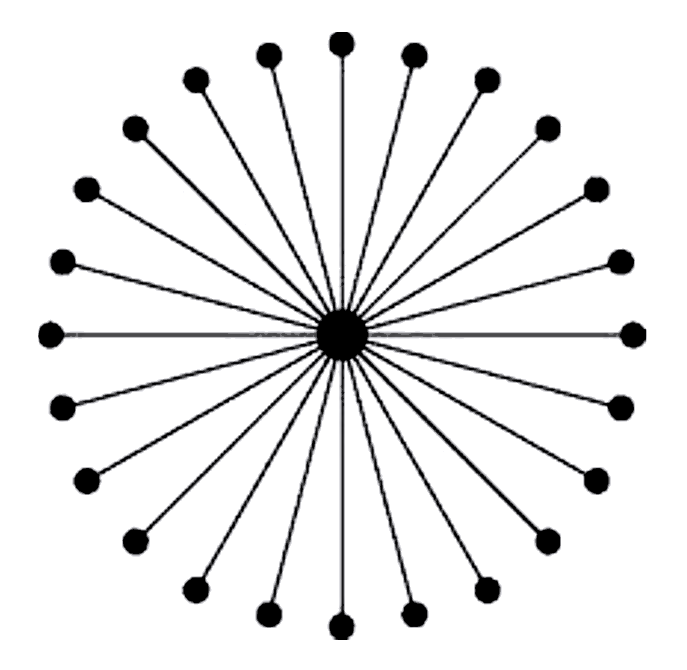
\includegraphics[width=7cm]{imagens/star.png}
    \caption{Um grafo de estrela, onde um vértice intermedia todas as interações.}
    \label{fig:star}
    \Fonte{\citeonline{Newman2010}}
\end{figure}

A centralidade por intermediação pode ser aplicada sem alterações em grafos dirigidos, visto que os arcos que ligam os vértices de um caminho devem ter origem no atual e destino no próximo da sequência. Além disso, a intermediação pode também ser aplicada em grafos ponderados, pois a definição de um caminho mínimo já leva em consideração o peso das ligações, conforme descrito na Seção \ref{sec:graphfoundation}.

\subsubsection{Proximidade} \label{sec:closeness}

A centralidade por proximidade (do inglês \textit{closeness}) caracteriza-se, conforme inicialmente definida por \citeonline{Bavelas1950}, como uma métrica de quão próximo o vértice em questão se encontra dos demais, sendo que a proximidade pode ser compreendida como o inverso da distância entre vértices. Concretamente, as distâncias são medidas através do cômputo de todos os caminhos mínimos com origem no vértice sob consideração e destino em cada um dos outros vértices do grafo (ou seja, $|V|$ caminhos).

\citeonline{Newman2010} interpreta a centralidade por proximidade como uma métrica que representa a facilidade de acesso à informação e influência direta sobre outros vértices. Já \citeonline{Grando2015} compreendem que a métrica caracteriza independência, pois vértices próximos dos demais não dependem dos outros para que possam se comunicar, influenciar ou atingir e serem atingidos de qualquer maneira por outros vértices do grafo.

Como seu cálculo depende intimamente de caminhos mínimos, a proximidade também pode ser aplicada em grafos dirigidos e ponderados, assim como a centralidade por intermediação, descrita na Seção \ref{sec:betweenness}. Entretanto, assim como na centralidade por grau, a proximidade também se desdobra em proximidade de entrada e de saída, pois a distância de um caminho de $u$ a $v$ pode ser diferente da distância de $v$ a $u$. Equação \ref{eq:incloseness} indica como a centralidade por proximidade de entrada é calculada para um vértice $v_k$ qualquer, enquanto a Equação \ref{eq:outcloseness} define a centralidade por proximidade de saída.

\begin{equation}
    \label{eq:incloseness}
    C_{P_{entrada}}(v_k) = \frac{|V|}{\sum_{i=1}^{|V|} d(v_i, v_k)}
\end{equation}

\begin{equation}
    \label{eq:outcloseness}
    C_{P_{saida}}(v_k) = \frac{|V|}{\sum_{i=1}^{|V|} d(v_k, v_i)}
\end{equation}

Nestas equações, $C_p$ expressa a centralidade por proximidade de entrada ou saída e $d(v_i, v_j)$ representa a distância do caminho mínimo com origem em $v_i$ e destino em $v_j$. O somatório das distâncias é situado no denominador para efetuar a inversão: quanto maior as distâncias, menor será o valor de centralidade por proximidade, e vice-versa. O numerador $|V|$ é utilizado para normalizar o resultado de acordo com o tamanho do grafo.

\subsubsection{Autovalor} \label{sec:eigenvector}

A centralidade por autovalor foi desenvolvida por \citeonline{Bonacich1987} como uma tentativa de aprimorar a centralidade por grau, definida na Seção \ref{sec:degree}. Segundo o autor, o grau de um vértice captura somente o número de vértices ligados a ele, sem levar em consideração quão importantes os mesmos são. Assim, a centralidade por autovalor caracteriza a importância de um vértice $u$ de forma recursiva -- isto é, conforme mais importantes os vértices ligados a $u$ forem, mais importante $u$ será. Desta maneira, um vértice pode ser importante tanto por estar ligado a um grande número de vértices quanto por estar ligado a poucos vértices cujas importâncias são elevadas.

Em essência, tem-se dois termos adicionais na função de centralidade por grau, que pode ser verificada nas Equações \ref{eq:indegree} e \ref{eq:outdegree}. O primeiro envolve a inclusão de um coeficiente constante ao somatório, habilitando sua normalização e assim tornando a equação mais genérica. O segundo, por sua vez, trata da seguinte modificação: ao invés de considerar somente o peso das ligações, adiciona-se uma multiplicação pela centralidade do vértice oposto, concretizando o conceito desta métrica \cite{Newman2010}. A Equação \ref{eq:eigenvector1} apresenta estas alterações.

\begin{equation}
    \label{eq:eigenvector1}
    C_A(v_k) = \frac{1}{r} \sum_{i=1}^{|V|} w(v_i, v_k) \cdot C_A(v_i) % talvez remover o \cdot
\end{equation}

É possível reescrever esta equação em termos da matriz de adjacências do grafo, definida na Seção \ref{sec:graphfoundation} e representada por $\mathbf{A}$, e tomar a função de centralidade por autovalor $C_a$ como um vetor com $|V|$ elementos, expresso por $\mathbf{x}$. Assim, tem-se:

\begin{equation}
    \label{eq:eigenvector2}
    \mathbf{x}_k = \frac{1}{r} \sum_{i=1}^{|V|} \mathbf{A}_{ki} \mathbf{x}_i
\end{equation}

Reordenando os termos e utilizando notação algébrica, é possível representar a Equação \ref{eq:eigenvector2} como $r\mathbf{x} = \mathbf{Ax}$, que é equivalente à equação de autovalores e autovetores da Álgebra Linear, onde o símbolo $\lambda$ é usualmente utilizado no lugar de $r$ \cite{Newman2010}. Segundo \citeonline{Bonacich1987} e \citeonline{Newman2010}, o maior autovalor da matriz de adjacências (conhecido como raio espectral) é utilizado como coeficiente devido a algumas de suas propriedades matemáticas. Assim, a centralidade por autovalor $C_a$ de um vértice de índice $k$ é dada por $\mathbf{x}_k$, onde $\mathbf{x}$ é o autovetor associado ao maior autovalor $r$.

Assim como a centralidade por grau, nenhuma alteração é necessária para tratar de grafos ponderados. No caso de grafos dirigidos, porém, além de existir o desdobramento em centralidade de entrada e de saída, ocorre uma segunda peculiaridade: vértices com centralidade zero -- um fenômeno que se manifesta quando o grau de entrada ou saída é zero -- podem, dependendo do padrão formado pelos arcos, causar uma reação em cadeia, fazendo com que um grande número de vértices do grafo também possuam centralidade zero, devido à multiplicação. Em algumas topologias, como em grafos acíclicos dirigidos, este efeito torna o uso da centralidade por autovalor impraticável \cite{Newman2010}.

Devido a estes fatores dificultantes, a centralidade por autovalor é geralmente aplicada em grafos não dirigidos. Uma métrica de centralidade similar, apropriada para aplicação em grafos dirigidos, é a centralidade de Katz, discutida na próxima seção.

\subsubsection{Katz} \label{sec:katz}

A centralidade de Katz, proposta por \citeonline{Katz1953}, caracteriza-se por possuir um conceito bastante similar à centralidade por autovalor (descrita na Seção \ref{sec:eigenvector}, sendo isenta de alguns dos seus problemas, mesmo tendo sido publicada anteriormente. Em relação à centralidade por autovalor, a principal mudança envolve a inclusão de uma centralidade base, sendo esta representada por uma constante $\beta$. Assim, a centralidade de um vértice nunca será zero, e portanto a propagação de importâncias de valor zero pelo grafo será inibida \cite{Newman2010}. Apesar disso, também é possível aplicar esta métrica em grafos não dirigidos, sem a necessidade de qualquer modificação.

Além disso, a centralidade de Katz adiciona um coeficiente $\alpha$ à equação, denominado fator de atenuação. \citeonline{Katz1953} propõe seu uso para modelar o fenômeno de perda de informação ou influência à medida que o vértice de destino se distancia da origem, passando por outros vértices no caminho. \citeonline{Newman2010} complementa observando que as duas constantes se contrapõem, sendo necessário encontrar um balanço entre a importância base e aquela advinda de contatos. Segundo o mesmo autor, ao definir-se $\alpha$ como 0, toda a importância recai sobre $\beta$ (base); por outro lado, valores que ultrapassam o limite do recíproco do raio espectral de $\mathbf{A}$ fazem com que o cálculo deixe de convergir.

Não existem muitas diretrizes para a escolha das constantes $\alpha$ e $\beta$ além dos limites mencionados para $\alpha$. No entanto, \citeonline{Newman2010} sugere que é possível manter $\beta$ em 1, por ser a identidade da multiplicação, e manipular apenas o valor de $\alpha$. A função da centralidade de Katz pode ser definida como:

\begin{equation}
    \label{eq:katz}
    C_K = \alpha \sum_{i=1}^{|V|} w(v_i, v_k) \cdot C_K(v_i) + \beta
\end{equation}

\noindent sendo esta definição baseada na Equação \ref{eq:eigenvector1}, com $C_K$ expressando a centralidade de Katz. É possível também inverter os argumentos da função $w$, que representa o peso da ligação, para utilizar os pesos de saída ao invés dos pesos de entrada, assim como nas centralidades por grau e proximidade; a equação completa foi omitida a favor da brevidade.

\subsection{Detecção de Comunidades} \label{sec:communities}

Redes complexas são assim denominadas devido aos padrões estruturais que podem ser observados ao estudá-las. Um padrão presente na grande maioria das redes complexas e que vem recebendo considerável interesse na literatura científica é a estrutura de comunidades\footnote{Tradução livre de \textit{community structure}.}, que consiste no agrupamento de vértices da rede em diversos módulos ou aglomerados \cite{Fortunato2016}.

Estes componentes, denominados \emph{comunidades} de agora em diante, consistem em grupos de vértices com alta concentração de ligações internas, apresentando algum nível de segregação (ou seja, poucas ligações) em relação a outras comunidades. A estrutura de comunidades é um exemplo de fenômeno observável exclusivamente em redes complexas, não se manifestando em grafos de outros tipos, como grafos aleatórios \cite{Fortunato2007}. A Figura \ref{fig:communitystructure} apresenta um exemplo de uma rede complexa que contém três comunidades, representadas pelos círculos tracejados, com uma aresta interligando-as.

\begin{figure}[ht]
    \centering
    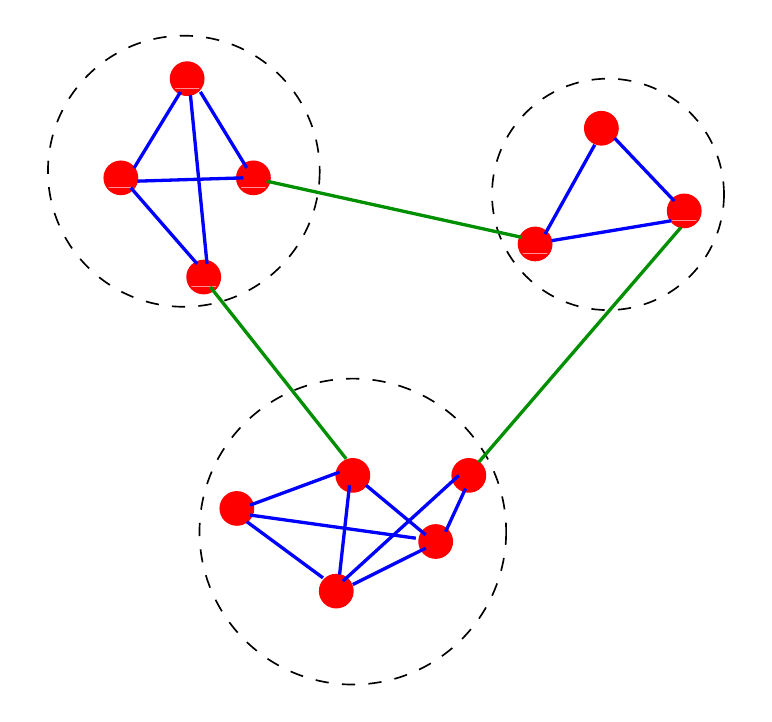
\includegraphics[width=8cm]{imagens/communities.png}
    \caption{Uma rede complexa simples composta por três comunidades.}
    \label{fig:communitystructure}
    \Fonte{\citeonline{Fortunato2010}}
\end{figure}

A identificação das comunidades que compõem uma rede provê a analistas uma visão mais sofisticada acerca de sua estrutura, fornecendo evidências sobre as funções dos grupos de vértices presentes na rede e de que forma estes grupos se comunicam. O processo também auxilia na análise da independência entre as comunidade da rede. Caso a rede não possua uma clara estrutura de comunidades, tal constatação caracteriza por si só uma importante informação sobre os aspectos da topologia da rede \cite{Newman2006}.

O estudo e a detecção de comunidades é de interesse prático em diversos domínios da ciência. Exemplos incluem a análise de páginas da \textit{web}, onde comunidades podem representar páginas que tratam de assuntos similares; a identificação de clientes com interesses similares, habilitando o desenvolvimento de sistemas de recomendação mais eficazes; o mapeamento de reações metabólicas e complexos de proteínas; o reconhecimento de indivíduos em redes criminosas; a identificação de componentes funcionais utilizados na percepção olfativa; entre outros \cite{Newman2006,Fortunato2010,Santiago2017}.

Segundo diversos autores, como \citeonline{Fortunato2007} e \citeonline{Newman2006}, a definição de comunidade não é totalmente exata e objetiva; geralmente, tem-se apenas uma noção intuitiva de seu conceito, envolvendo uma densidade elevada de ligações entre os vértices de uma comunidade (intra-comunidade) e poucas ligações entre vértices de comunidades diferentes (inter-comunidade). Cliques, definidos na Seção \ref{sec:graphfoundation}, são exemplos claros de comunidades; entretanto, dada sua raridade em redes complexas de tamanho razoável, considera-se que sua definição é muito rígida para ser adotada como um modelo prático de comunidade \cite{Fortunato2007}.

Sendo assim, algumas definições matemáticas foram desenvolvidas, as quais, em sua grande maioria, buscam avaliar a qualidade da divisão de uma rede complexa em comunidades. Com isso, torna-se possível identificá-las através de um processo de otimização matemática. Duas destas definições, que angariaram considerável popularidade na literatura, serão apresentadas nas próximas seções.

\subsubsection{Modularidade} \label{sec:modularity}

A otimização da função de Modularidade, desenvolvida por \citeonline{Newman2004}, é considerada a forma mais popular de efetuar o processo de detecção de comunidades por \citeonline{Fortunato2010}. A função é baseada no conceito da ausência da estrutura de comunidades em grafos aleatórios; sendo assim, define-se um ``modelo nulo''\footnote{Tradução livre de \textit{null model}}, que consiste em uma cópia da rede original porém com suas ligações redefinidas, buscando eliminar a estrutura de comunidades.

Após o estabelecimento do modelo nulo, computa-se a diferença entre a rede original, com seus vértices agrupados de alguma maneira, e seu modelo nulo. Caso não haja diferença, considera-se que o agrupamento dos vértices possui baixa qualidade -- isto é, não revela a estrutura de comunidades da rede. Por outro lado, se a diferença for elevada, então o agrupamento sob avaliação é tomado como um particionamento de alta qualidade da rede em suas comunidades \cite{Fortunato2010}.

O modelo nulo adotado com maior frequência envolve uma redefinição das ligações de forma a manter a distribuição de graus dos vértices da rede. Sendo assim, para um vértice $u$ qualquer, seu grau tende a ser igual ou similar no modelo nulo, porém o conjunto de vértices aos quais $u$ está conectado tende a ser totalmente diferente. Matematicamente, a probabilidade de dois vértices $u$ e $v$ estarem conectados no modelo nulo é dada por $\frac{k_uk_v}{2m}$, onde $k_u$ representa o grau do vértice $u$ e $m$ expressa o número de ligações presentes na rede. Com isso, define-se a função de Modularidade como:

\begin{equation}
    \label{eq:modularity}
    Q = \frac{1}{2m}\sum_{i=1}^{|V|}\sum_{j=1}^{|V|} \left [ \left ( A_{ij} - \frac{k_ik_j}{2m} \right ) \delta(C_i, C_j) \right ]
\end{equation}

\noindent onde $Q$ representa a função de Modularidade, $m$ representa o número de ligações da rede, $A$ expressa sua matriz de adjacências, $k_i$ simboliza o grau do vértice $i$ e a função $\delta(C_i, CC_j)$ possui valor 1 caso os vértices $i$ e $j$ pertençam à mesma comunidade e 0 caso contrário. A função $Q$ também pode ser trivialmente adaptada para grafos dirigidos e ponderados \cite{Fortunato2010}.

A detecção de comunidades através da otimização da função de Modularidade pertence à classe de problemas NP-difíceis, e portanto demanda esforço computacional extremamente elevado, sendo impraticável em redes complexas de tamanho razoável \cite{Brandes2008}. Para tratar desta característica, diversos métodos heurísticos foram desenvolvidos recentemente \cite{Blondel2008,Santiago2017,Nascimento2013,Agarwal2008,Pizzuti2008}.

Além disso, \citeonline{Fortunato2007b} identificaram que a detecção de comunidades por otimização da Modularidade apresenta um problema denominado ``resolução limite'', pelo qual a Modularidade tende a avaliar com maior qualidade agrupamentos de uma rede cujas comunidades são compostas por mais vértices. Sendo assim, o método é incapaz de identificar comunidades pequenas em redes razoavelmente grandes, mesmo quando tais comunidades são altamente coesas e esparsamente ligadas.

Um exemplo deste fenômeno é apresentado na Figura \ref{fig:ringofcliques}, onde uma rede composta por 16 cliques (cada qual contendo 4 vértices), conectados entre si por uma aresta, tem seu agrupamento ótimo consistindo em 8 comunidades de 2 cliques cada uma, ao invés do agrupamento esperado de 16 comunidades, com cada clique pertencendo à sua própria comunidade.

\begin{figure}[ht]
    \centering
    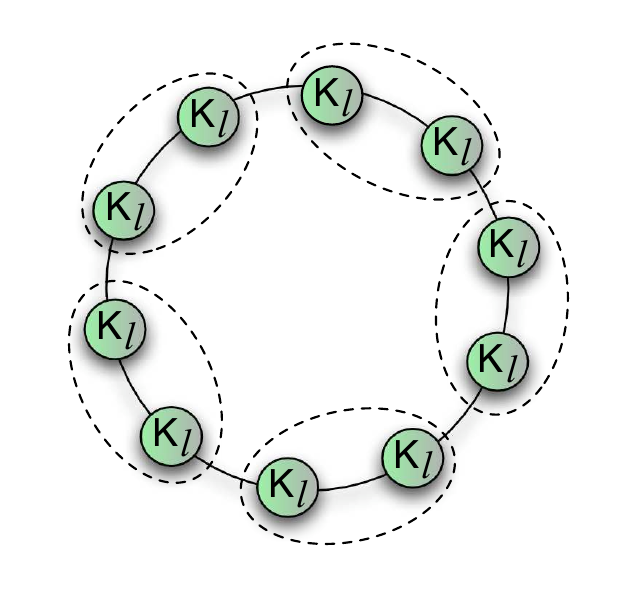
\includegraphics[width=9cm]{imagens/ring_of_cliques.png}
    \caption{Anel de cliques.}
    \label{fig:ringofcliques}
    \Fonte{\citeonline{Fortunato2010}}
\end{figure}

Uma função alternativa à Modularidade, desenvolvida com a intenção de contornar este problema, é apresentada na seção seguinte.

\subsubsection{Modularidade por Densidade} \label{sec:density}

Buscando solucionar os problemas associados à Modularidade apontados por \citeonline{Fortunato2007b}, \citeonline{Li2008} propuseram uma adaptação denominada Modularidade por Densidade. Nesta formulação, o número de vértices que compõem cada comunidade é utilizado para normalizar o resultado da equação, ao invés do número total de ligações do grafo como na Modularidade (conforme pode-se observar na Equação \ref{eq:modularity}.

Além disso, a utilização de um modelo nulo é substituída por um termo alternativo, que envolve o cômputo da diferença entre o número de ligações internas, com origem e destino em vértices da mesma comunidade, e ligações externas, com origem em vértices da comunidade atual e destino em vértices de outras comunidades \cite{Li2008,Santiago2017}. Em sua forma mais simples, a função de Modularidade por Densidade pode ser definida da seguinte maneira:

\begin{equation}
    \label{eq:density1}
    D = \sum_{C \in P} \left ( \frac{4|E_C| - \sum_{u \in C} k_u}{|C|} \right )
\end{equation}

\noindent onde $D$ simboliza a Modularidade por Densidade e $P$ representa o conjunto de comunidades, sendo cada comunidade expressa por $C$. Assim, para uma comunidade $C$ qualquer, $|C|$ indica o número de vértices que a compõem e $|E_C|$ representa o número de arestas internas à mesma. O termo $\sum_{u \in C} k_u$ consiste em um somatório dos graus dos vértices da comunidade, representando assim a densidade de ligações externas.

Usualmente, a Modularidade por Densidade é utilizada em sua variação paramétrica, que permite definir se é preferível identificar comunidades de tamanho pequeno ou grande. A Equação \ref{eq:density2} apresenta esta variação, onde o parâmetro $\lambda \in [0, 1]$ pode ser reduzido para encontrar comunidades menores ou aumentado para encontrar comunidades de porte maior. Caso o mesmo seja mantido em seu valor intermediário de 0,5, a função se comportará da mesma forma que a Equação \ref{eq:density1} \cite{Li2008,Santiago2017}. Nesta formulação, a função $g(C)$ representa o termo de ligações externas dado por $\sum_{u \in C} k_u$.

\begin{equation}
    \label{eq:density2}
    D_{\lambda} = \sum_{C \in P} \left ( \frac{4\lambda|E_C| - (2 - 2\lambda) (g(C) - 2|E_C|) }{|C|} \right )
\end{equation}

Assim como a Modularidade, a detecção de comunidades através da otimização da Modularidade por Densidade também demanda alto esforço computacional e, portanto, também é tipicamente utilizada em conjunto com métodos heurísticos. Exemplos incluem os algoritmos desenvolvidos por \citeonline{Gong2012}, \citeonline{Santiago2017} e \citeonline{KarimiMajd2015}.